\chapter{Release 1}
\addcontentsline{toc}{chapter}{Release 1}
\markboth{Release 1}{Release 1}
\renewcommand\fbox{\fcolorbox{blue}{white}}
\label{chap:release1}
% section starts from 1 
%\minitoc

\section*{Introduction}

Ce chapitre présente la première version de notre application. Il est composé de cinq sprints qui ont été réalisés en 10 semaines. Nous avons commencé par la conception de l'application, puis nous avons implémenté les fonctionnalités de base de l'application tels que la gestion des documents et des signatures. Dans ce chapitre, nous décrirons en détail les fonctionnalités de chaque sprint, les défis que nous avons rencontrés et les solutions que nous avons apportées pour les surmonter.

Release 1 : (Du 8 Février Au 19 Avril)

\fbox{\begin{minipage}{30em}
  \textbf{Organisation des sprints :} \\
  Cette release contient les cinq sprints:
  \begin{itemize}
    \item \textbf{Sprint 1:} Préparation de l'environnement du travail et étude de la solution.
    \item \textbf{Sprint 2:} Gestion des signatures.
    \item \textbf{Sprint 3:} Gestion des documents.
    \item \textbf{Sprint 4:} Visualisation et signature de fichiers.
    \item \textbf{Sprint 5:} Gestion du Profile.
  \end{itemize}
\end{minipage}}

\section{Sprint 1 (Préparation de l'environnement du travail et étude de la solution)}

\subsection{Sprint Goal}
L'objectif de ce sprint est de préparer l'environnement de travail et d'étudier la solution ainsi que les technologies à utiliser.

\subsection{Sprint Backlog}

%  4 columns table
% \begin{adjustwidth}{-1cm}{}
%   % \usepackage{longtable}
%     \begin{longtable}{|c|c|c|c|}
%       % \centering
%       \hline
%       \textbf{Les items} & \textbf{Les tâches} & \textbf{Période} & \textbf{Sprint} \\
%       \hline
%       % Numbered list
%       % \begin{enumerate}
%       %   \item Se former en Elise
%       %   % \item Se former en développement mobile avec Ionic Vue et Capacitor.
%       %   % \item Installer et Configurer l'environnement de développement. 
%       % \end{enumerate}
%       \noindent 1 & 1 & 1 & \vspace{-\baselineskip}
%       \begin{itemize}[label={--},noitemsep,leftmargin=*,topsep=0pt,partopsep=0pt]
%         \item Rechercher des informations sur les langages et les progiciels utilisé.
%         % \item Suivre une formation préparée par la société sur Elise.
%         % \item Suivre une formation sur Youtube qui explique les notions de base d'Ionic.
%         % \item Suivre une formation sur Youtube qui explique les notions de base du Capacitor.
%         % \item Suivre une formation sur Youtube qui explique les notions de base du Soap.
%         % \item Suivre une formation sur Youtube qui explique les notions de base du .NET core 6.
%         % \item Installer VS code.
%         % \item Installer Android Studio.
%         % \item Installer .NET Core 6 .
%         % \item Installer Ionic Version6.
%         % \item Installer Vue Js Version 3.
%         % \item Installer Capacitor Version 4.
%         % \item Télécharger SoapUi.
%         % \item \textbf{Application 1} Développer une application mobile qui consomme le webservice soap pour afficher les données de la météo 
%         % \item \textbf{Application 2} Développer une application mobile qui permet la création d'une signature.
%         % \item \textbf{Application 3} Développer une application mobile qui permet de visualiser un fichier PDF. 
%         % \item \textbf{Application 4} Développer une application mobile qui permet de signer un fichier PDF en utilisant les deux solutions 2 et 3.
%       \end{itemize} \\
%       % & 1\\

%       \end{longtable}
% \end{adjustwidth}

% \renewcommand*{\arraystretch}{1.8}
\begin{longtable}{|p{4cm}|p{7cm}|p{2cm}|p{2cm}|}
  \hline
  \textbf{Les items} &\textbf{Les tâches} & \textbf{Période} & \textbf{Sprint} \\
  \hline
  \vspace{-\baselineskip}
  \begin{enumerate}
    \setcounter{enumi}{1}
    \itemsep0em 
      \item Se former en Elise
      \item Se former en développement mobile avec Ionic Vue et Capacitor.
      \item Installer et Configurer l'environnement de développement. 

  \end{enumerate}
  &
  \vspace{-\baselineskip}
  \begin{itemize}
    \itemsep0em 
    \item Suivre une formation préparée par la société sur Elise.
    \item Suivre une formation sur Youtube qui explique les notions de base d'Ionic.
    \item Suivre une formation sur Youtube qui explique les notions de base du Capacitor.
    \item Suivre une formation sur Youtube qui explique les notions de base du Soap.
    \item Suivre une formation sur Youtube qui explique les notions de base du .NET core 6.
    \item Installer VS code.
    \item Installer Android Studio.
    \item Installer .NET Core 6 .
    \item Installer Ionic Version6.
    \item Installer Vue Js Version 3.
    \item Installer Capacitor Version 4.
    \item Télécharger SoapUi.
    \item \textbf{Application 1} Développer une application mobile qui consomme le webservice soap pour afficher les données de la météo 
    \item \textbf{Application 2} Développer une application mobile qui permet la création d'une signature.
    \item \textbf{Application 3} Développer une application mobile qui permet de visualiser un fichier PDF. 
    \item \textbf{Application 4} Développer une application mobile qui permet de signer un fichier PDF en utilisant les deux solutions 2 et 3.
  \end{itemize}
  &
  De 8 à 15 février  
  &
  1
  \\
  \hline
  \caption{Product Backlog Sprint 1}


\end{longtable}

\subsection{Sprint Review}
Suite à cette Technical Story, nous avons préparé notre environnement de travail où nous aurons les possibilités de terminer les prochains sprints.

\subsection{Sprint Retrospective}

\begin{itemize}
  \item \textbf{Ce qui a bien fonctionné :}
  \begin{itemize}
    \item Nous avons pu suivre les formations préparées par la société.
    \item Nous avons pu suivre les formations sur Youtube.
    \item Nous avons pu installer les outils nécessaires pour le développement.
    \item Nous avons bien mis nos connaissances en pratique dans certains projets préparatoires (Application 1, 2, 3 et 4).
  \end{itemize}
  \item \textbf{Ce qui n'a pas bien fonctionné :}
  
  Nous avons remarqué que le temps de formation est très réduit, nous avons donc décidé de suivre des formations sur Youtube pour nous former sur les technologies à utiliser en plus de la formation préparée par la société.
\end{itemize}

\section{Sprint 2 (Gestion des signatures)}

\subsection{Sprint Goal}

L'objectif de ce sprint est de développer et mettre en place un système de gestion des signatures permettant aux utilisateurs d'ajouter et de visualiser facilement les signatures crée, tout en garantissant la sécurité.

\pagebreak
\subsection{Sprint Backlog}

\begin{longtable}{|p{4cm}|p{7cm}|p{2cm}|p{2cm}|}
  \hline
  \textbf{Les items} &\textbf{Les tâches} & \textbf{Période} & \textbf{Sprint} \\
  \hline
  \vspace{-\baselineskip}
  \begin{enumerate}
    \setcounter{enumi}{1}
    \itemsep0em 
      \item Créer une signature.
      \item Supprimer d'une signature.
      \item Visualiser une signature.

  \end{enumerate}
  &
  \vspace{-\baselineskip}
  \begin{itemize}
    \itemsep0em 
    \item Préparer les interfaces sur Figma.
    \item Développer une interface pour créer et lister les signatures
    \item Développer une interface pour visualiser la signature.
    \item Développer la fonction qui permet de créer une signature.
    \item Développer la fonction qui permet de lister les signatures.
  \end{itemize}
  &
  De 8 à 15 février  
  &
  2
  \\
  \hline
  \caption{Product Backlog Sprint 2}


\end{longtable}

\subsection{Implémentation du Sprint 2}
\textbf{•	Diagramme de cas d'utilisation du sprint 2 : « Gestion des signatures »}

% add image
\begin{figure}[h]
  \centering
  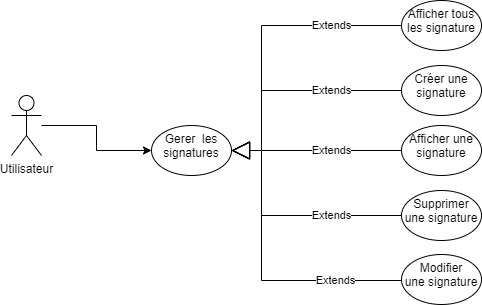
\includegraphics[width=0.8\textwidth]{use_case_signature_sprint_2}
  \caption{Diagramme de cas d'utilisation du sprint 2 : « Gestion des signatures »}
  \label{fig:UseCaseDiagram}
\end{figure}

\subsubsection{Analyse des besoins:}
\textbf{•	Description textuelle de cas d'utilisation « Créer une signature »}

\begin{longtable}{|p{5cm}|p{10cm}|}
\hline
\textbf{Cas d'utilisation}&Créer une signature\\
\hline
\textbf{Acteurs}&Utilisateur\\
\hline
\textbf{Pré Condition}&L'utilisateur doit être authentifié\\
\hline
\textbf{Post Condition}&Création d'une signature\\
\hline
\textbf{Scénario Nominal}&
\vspace{-\baselineskip}
\begin{enumerate}
    \setcounter{enumi}{1}
  \item L'utilisateur dessine sa signature sur le pad.
  \item L'utilisateur clique sur le bouton enregistrer.
  \item L'utilisateur entre le nom de la signature.
  \item L'utilisateur clique sur le bouton enregistrer.
  \item Le système affiche un message de succès.
\end{enumerate}\\
\hline
\textbf{Scénario Alternatif}&
\vspace{-\baselineskip}
\begin{enumerate}
    \setcounter{enumi}{2}
    \item Aucun résultat.
    \item L'utilisateur ajoute une signature d'après l'OCR.
    \item Le système affiche un message d'erreur pour s'assurer de signer
    \item Le système affiche un message d'erreur pour s'assurer d'entrer le nom
\end{enumerate}\\
\hline
\textbf{Scénario d'exception}&Erreur de connexion\\
\hline
\end{longtable}

\textbf{Terminologie paragraphe :} \\
\textbf{OCR :} signifie Optical Character Recognition (reconnaissance optique de caractères en français). Il s'agit d'un processus de conversion d'images numérisées de textes en fichiers éditables et interprétables par des ordinateurs.
  

\textbf{•	Description textuelle de cas d'utilisation « Supprimer  une signature »}

\begin{longtable}{|p{5cm}|p{10cm}|}
\hline
\textbf{Cas d'utilisation}&Supprimer une signature\\
\hline
\textbf{Acteurs}&Utilisateur \\
\hline
\textbf{Pré Condition}&L'utilisateur doit être authentifié\\
\hline
\textbf{Post Condition}&Suppression  d'une signature\\
\hline
\textbf{Scénario Nominal}&
\vspace{-\baselineskip}
\begin{enumerate}
    \setcounter{enumi}{1}
    \item L'utilisateur clique sur le bouton supprimer.
    \item Le système affiche une alerte de vérification.
    \item L'utilisateur clique sur le bouton confirme.
    \item La signature est supprimer de la base.
    \item Le système affiche un message de succès.
\end{enumerate}\\
\hline
\textbf{Scénario d'exception}&Erreur de connexion\\
\hline
\end{longtable}

\textbf{•	Description textuelle de cas d'utilisation « Visualiser une signature »}

\begin{longtable}{|p{5cm}|p{10cm}|}
\hline
\textbf{Cas d'utilisation}&Visualiser une signature\\
\hline
\textbf{Acteurs}&Utilisateur \\
\hline
\textbf{Pré Condition}&L'utilisateur doit être authentifié\\
\hline
\textbf{Post Condition}&Visualisation d'une signature\\
\hline
\textbf{Scénario Nominal}&
\vspace{-\baselineskip}
\begin{enumerate}
    \setcounter{enumi}{1}
    \item L'utilisateur clique sur le bouton visualiser.
    \item Le système affiche la signature.
\end{enumerate}\\
\hline
\textbf{Scénario d'exception}&Erreur de connexion\\
\hline
\end{longtable}

\subsubsection{Analyse détaillée}
La présentation de démarche d'analyse fonctionnelle d'un sprint est très importante pour la satisfaction d'un client parce qu'elle consiste à caractériser les fonctions offertes par un produit.
Donc, nous allons faire l'analyse des différents cas d'utilisation en utilisant le diagramme de classes d'analyse.

//TODO: ADD DIAGRAMME DE CLASSE ANALYSE
// TODO: ADD DIAGRAMMEs

\subsubsection{Conception}

Après la présentation des diagrammes d'analyse de CU, nous avons présenté dans cette partie le diagramme de classe de conception de CU d'user story 1.

\textbf{•	Diagramme de classe de conception de CU d'user story 1 : « Gestion des signatures »}

% add image
\begin{figure}[h]
  \centering
  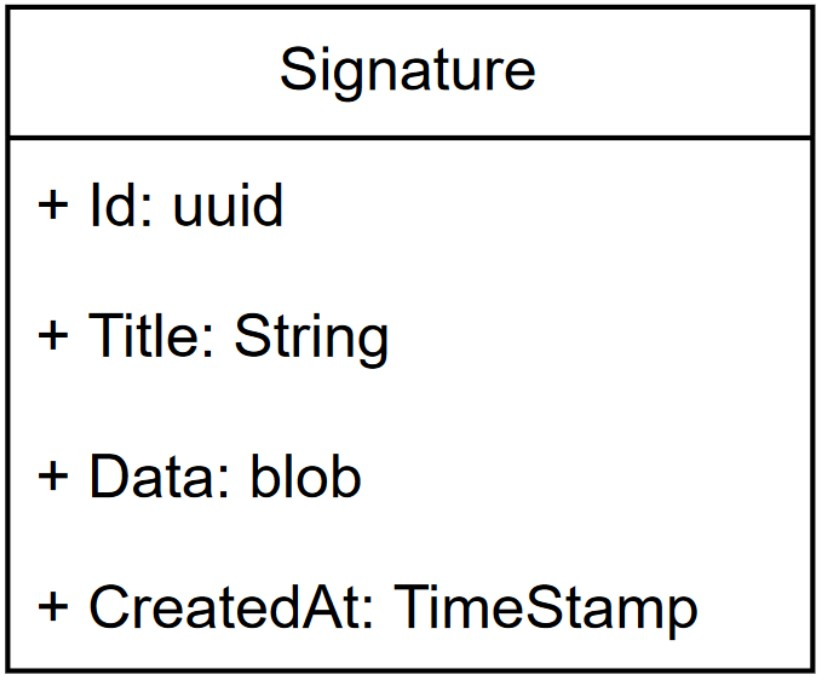
\includegraphics[width=0.4\textwidth]{class_diagram_signatures}
  \caption{Diagramme de classe de conception de CU d'user story 1 : « Gestion des signatures »}
  \label{fig:UseCaseDiagramSignatures}
\end{figure}

\subsubsection{Réalisation}

Après la présentation des diagrammes d'analyse de CU, nous avons présenté dans cette partie des captures d'écran de l'application.

\textbf{•	Interface de création d'une signature:}

Cette capture d'écran, représente l'interface de création d'une signature par un utilisateur

% add image
\begin{figure}[h]
  \centering
  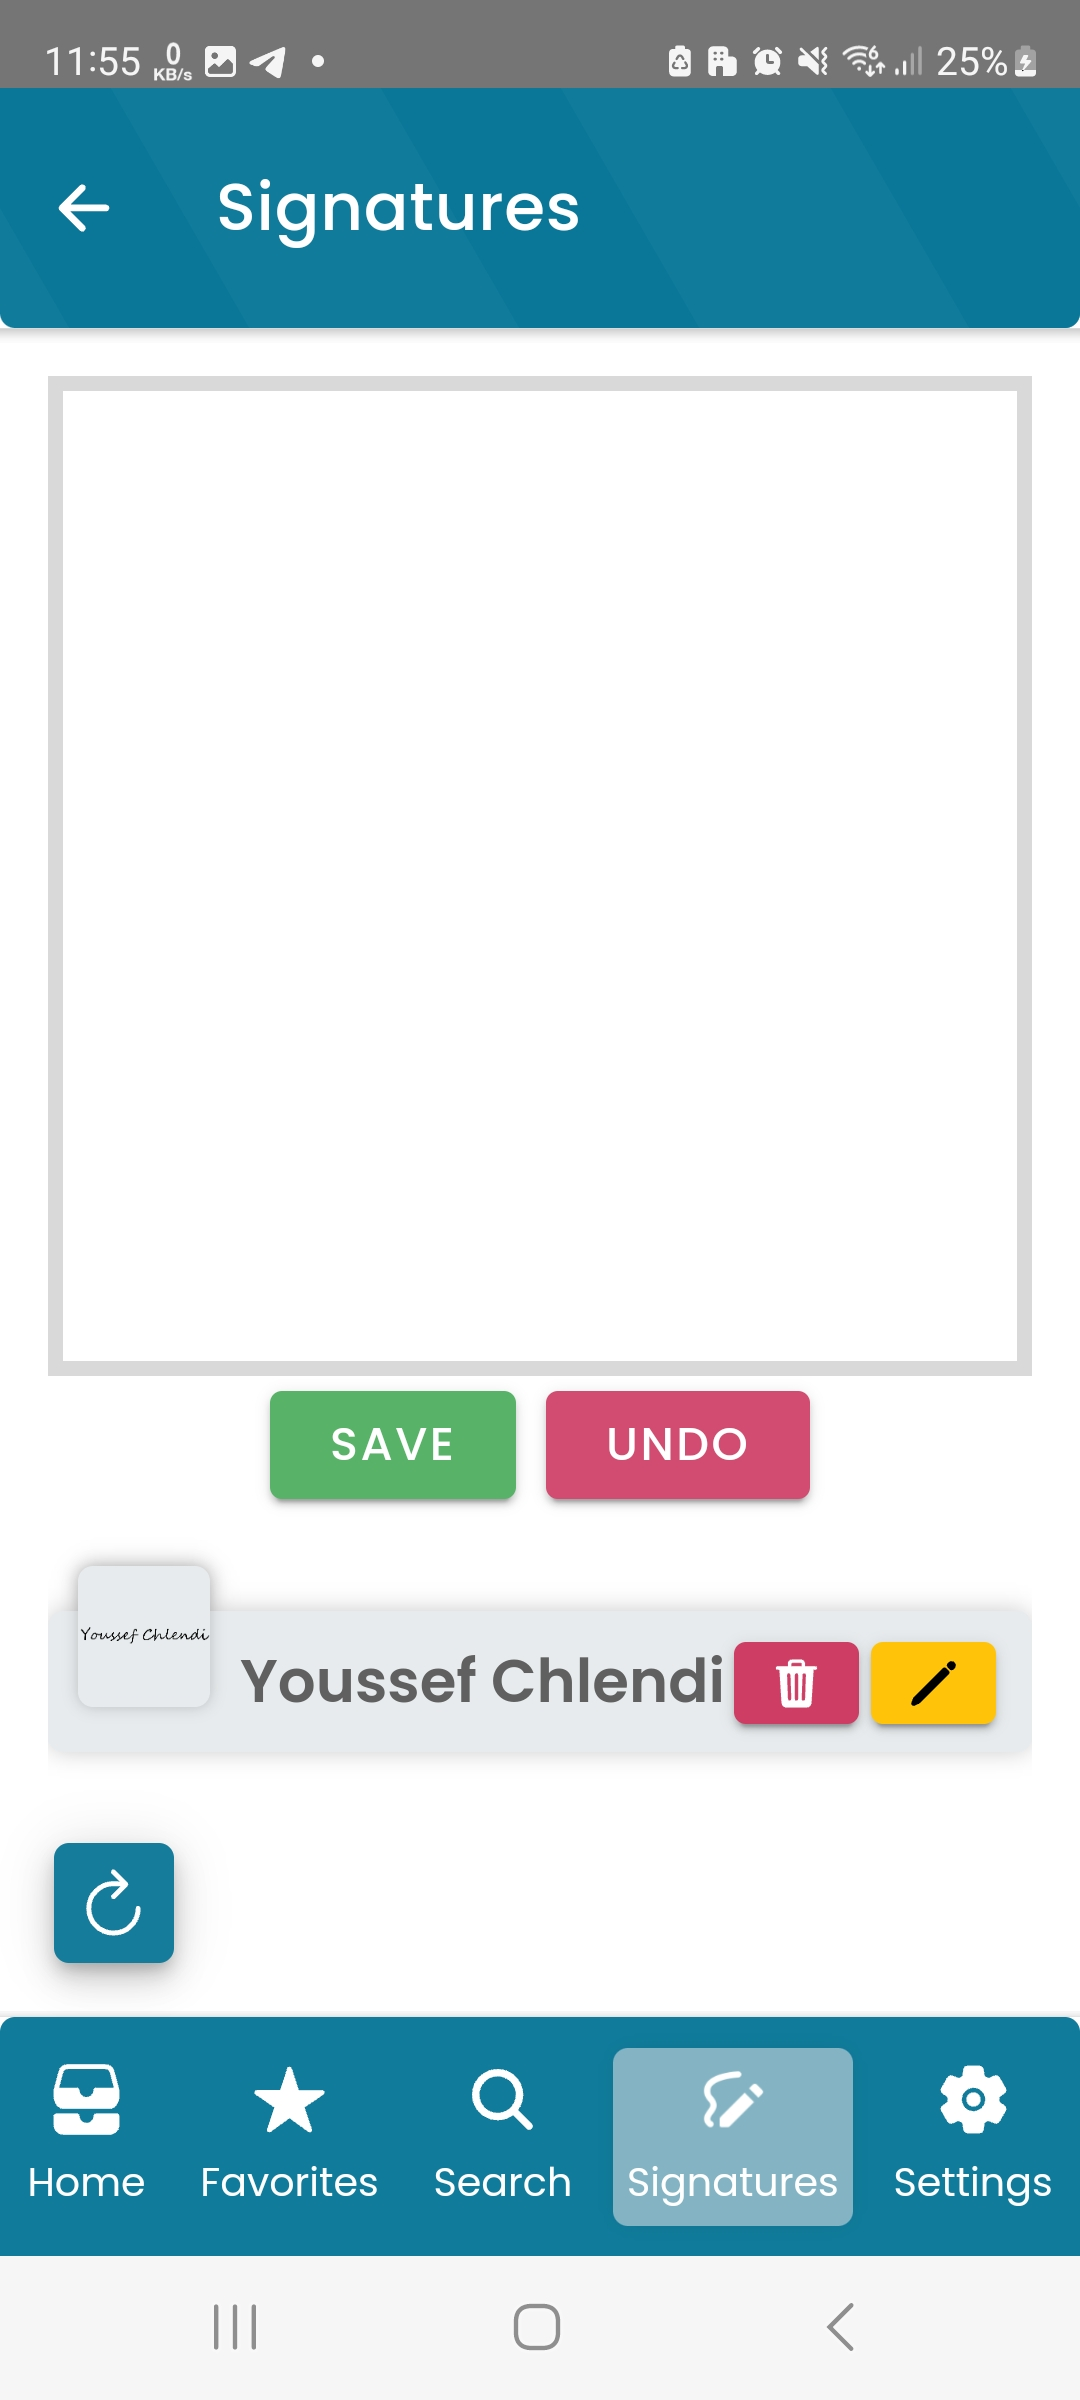
\includegraphics[width=0.3\textwidth,keepaspectratio=true, height=0.3\textheight]{signature_creation}
  \caption{Interface de création d'une signature}
  \label{fig:signature_creation}
\end{figure}

\textbf{•	Signer puis cliquer sur « save » : Interface de saisie du titre:}\\
Cette capture d'écran, représente l'interface de saisie du titre de la signature par un utilisateur
% add image
\begin{figure}[h]
  \centering
  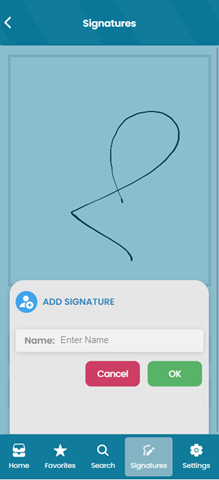
\includegraphics[width=0.3\textwidth,keepaspectratio=true, height=0.3\textheight]{signature_form}
  \caption{Interface de saisie du titre de la signature}
  \label{fig:signature_title}
\end{figure}

\textbf{•	Interface de visualisation d'une signature:}\\
Cette capture d'écran, représente l'interface de visualisation d'une signature par un utilisateur

\newpage

% add image
\begin{figure}[h]
  \centering
  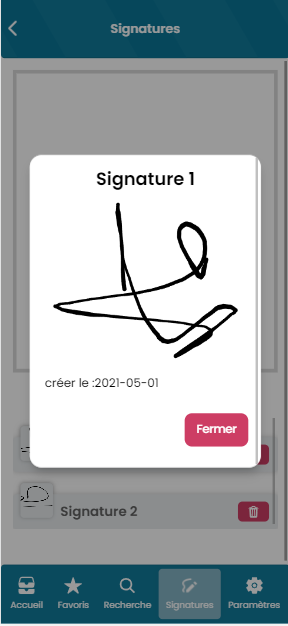
\includegraphics[width=0.3\textwidth,keepaspectratio=true, height=0.3\textheight]{signature_preview}
  \caption{Interface de visualisation d'une signature}
  \label{fig:signature_view}
\end{figure}

\textbf{•	Interface de suppression d'une signature:}\\
Cette capture d'écran, représente l'interface de suppression d'une signature par un utilisateur

% add image
\begin{figure}[h!]
  \centering
  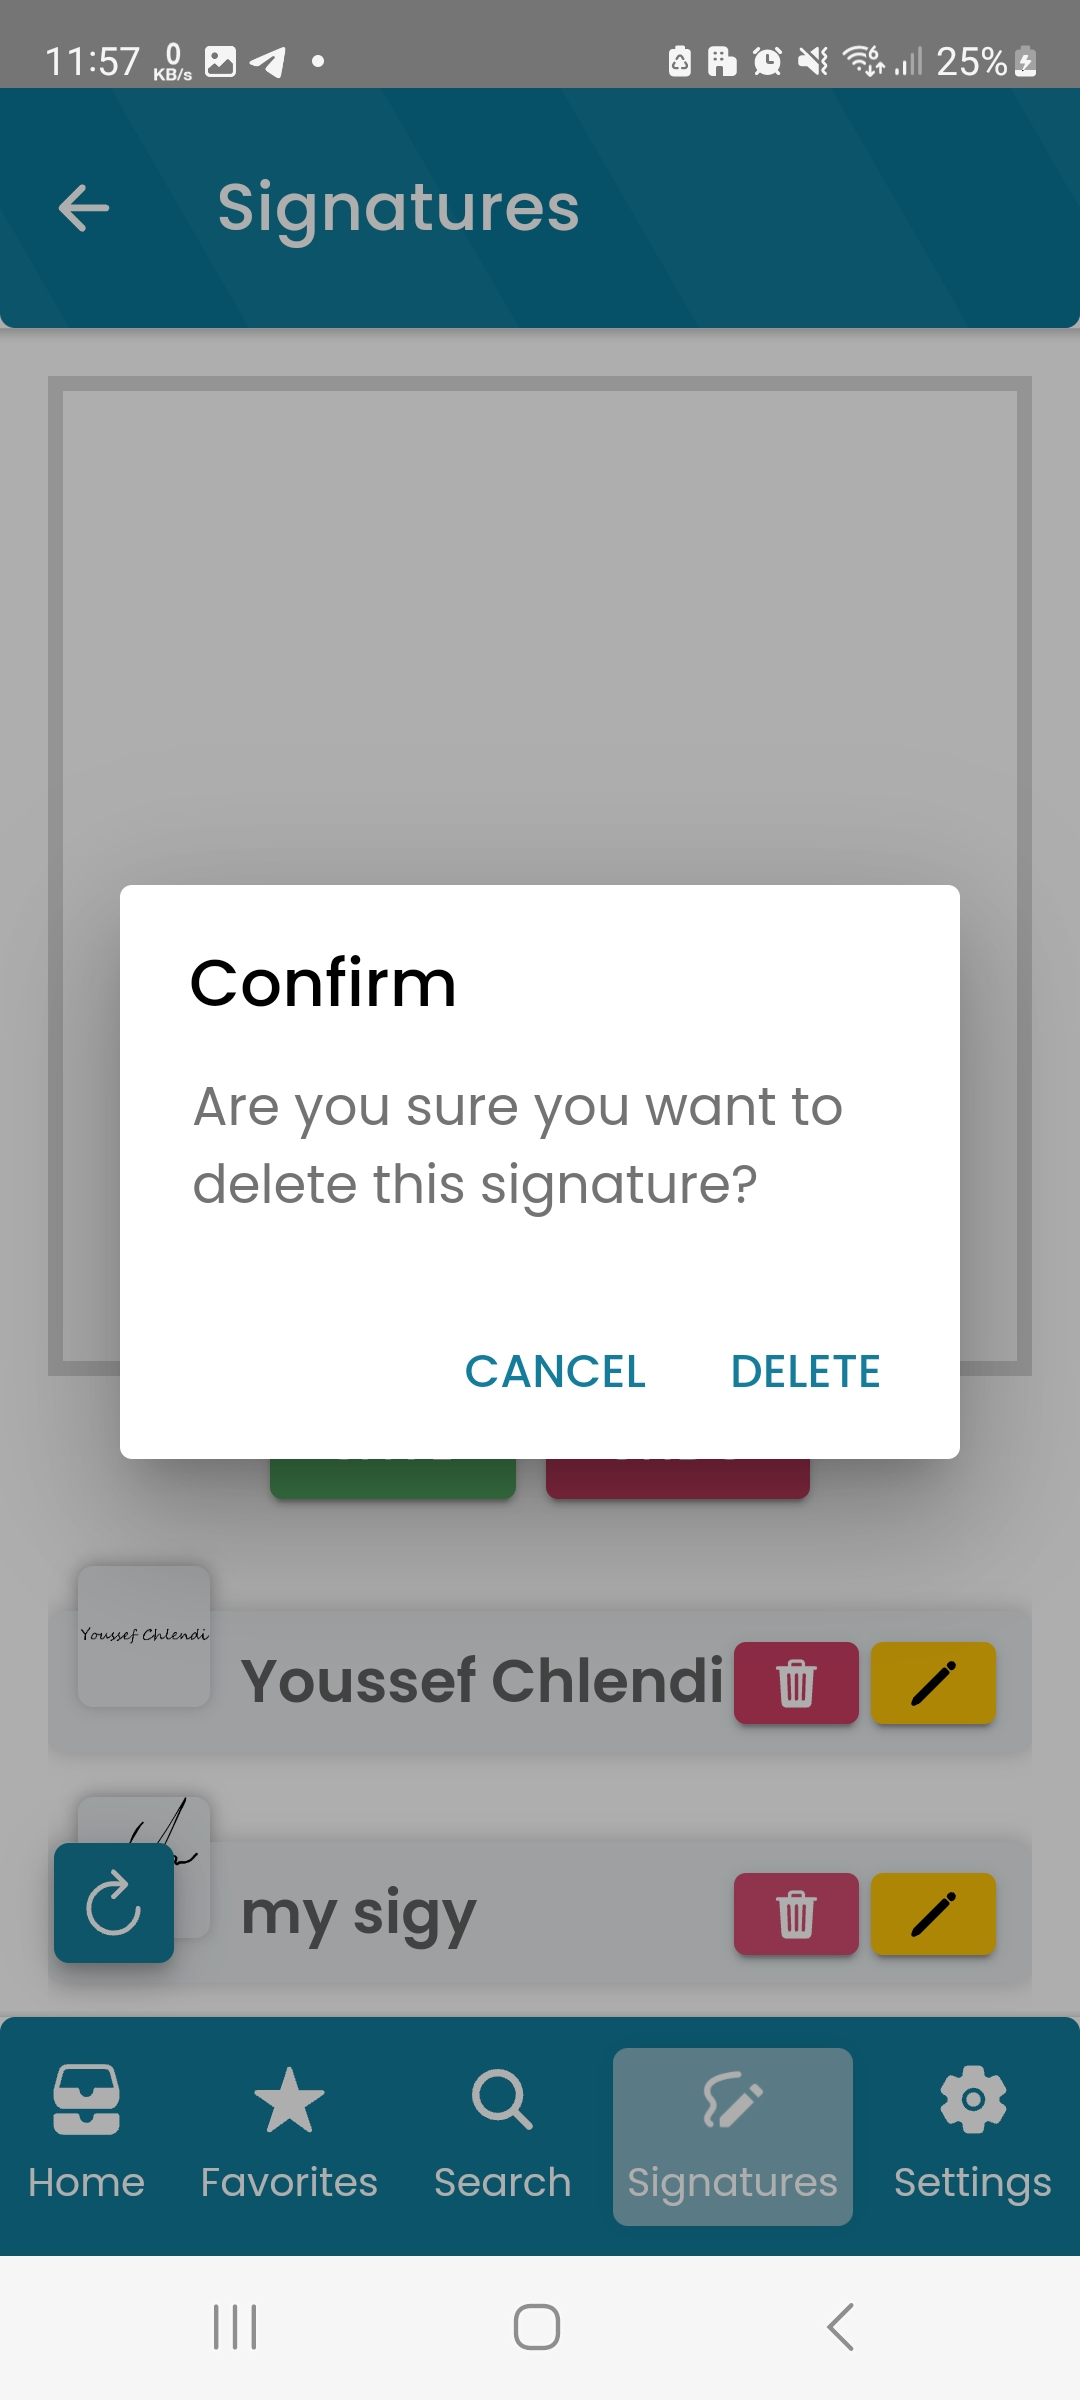
\includegraphics[width=0.3\textwidth,keepaspectratio=true, height=0.3\textheight]{signature_delete}
  \caption{Interface de suppression d'une signature}
  \label{fig:signature_delete}
\end{figure}



\subsection{Sprint review:}
A la fin de ce sprint, nous avons planifié une réunion dans la société Neoledge afin de vérifier notre démarche de travail par rapport au besoin de client tout en respectant le délai que nous avons prévu.

Nous avons fait une démonstration durant laquelle nous allons présenter notre incrément :

\begin{itemize}
  \item La création d'une signature.
  \item La visualisation de la signature.
  \item La suppression de la signature.
\end{itemize}

\subsection{Sprint retrospective:}

Après la Sprint Review, nous avons réfléchi à des pistes pour améliorer la qualité et l'efficacité de notre application.

\noindent\textbf{•	Ce qui s'est bien passé :}
\begin{itemize}
  \item Nous avons bien partagé les tâches entre nous à travers le logiciel Azure DevOps. 
  \item Nous avons terminé le sprint dans le délai.
\end{itemize}

\noindent\textbf{•	Ce qui s'est mal passé :}
\begin{itemize}
  \item L'intégration du bibliothèque vue-signature-pad
  \item Un problème rencontré lors de la sauvegarde de la signature était que l'image enregistrée occupait la totalité de l'espace du pad, ce qui nécessitait ensuite une étape de découpe pour obtenir uniquement la partie signée.
\end{itemize}

